\documentclass[12pt,a4paper]{article}

\usepackage{minted}
\usepackage[T1]{fontenc}
\usepackage{url}
\usepackage{color,soul}
\usepackage{caption}
\usepackage{biblatex}
\usepackage{float}
\usepackage{geometry}
\usepackage{times}
\usepackage{titlesec}
\usepackage{ragged2e}
\usepackage{fancyhdr}
\usepackage{pdfpages}
\usepackage{graphicx}
\usepackage{indentfirst}

\graphicspath{ {./images/} }

\AddToHook{cmd/section/before}{\clearpage}

\titleformat*{\section}{\fontsize{14}{10}\bfseries\selectfont\MakeUppercase}
\titleformat*{\subsection}{\fontsize{13}{10}\bfseries\selectfont}

\geometry{
    a4paper,
    left=35mm,
    right=25mm,
    top=25mm,
    bottom=30mm,
}

\pagestyle{fancyplain}
\fancyhf{}
\fancyfoot[R]{\thepage}
\renewcommand{\headrulewidth}{0pt}

\renewcommand{\baselinestretch}{1.5}

\captionsetup[table]{name=Tabela}
\captionsetup[figure]{name=Obrazek}
\renewcommand*\contentsname{Spis treści}
\renewcommand{\listtablename}{Spis tabel}
\renewcommand{\listfigurename}{Spis obrazków, fotografii}

\newfloat{code}{h}{loa}
\captionsetup[code]{name=Program}

\makeatletter
\renewcommand\listoffigures{
    \subsection*{\listfigurename
        \@mkboth{
           \MakeUppercase\listfigurename}{\MakeUppercase\listfigurename}}
    \@starttoc{lof}
}
\renewcommand\listoftables{
    \subsection*{\listtablename
        \@mkboth{
           \listtablename}{\listtablename}}
    \@starttoc{lot}
}
\renewcommand*{\listof}[2]{%
  \@ifundefined{ext@#1}{\float@error{#1}}{%
    \@namedef{l@#1}{\@dottedtocline{1}{1.5em}{2.3em}}%
    \subsection*{#2}% \float@listhead{#2}
    \begingroup\setlength{\parskip}{\z@}%
      \@starttoc{\@nameuse{ext@#1}}%
    \endgroup}
}
\makeatother

\addbibresource{sources.bib}

\title{Konstrukcja stacji pogodowej opartej na mikrokontrolerze ESP32 z interfejsem użytkownika oraz API REST}
\author{Szymon Uglis}

\begin{document}

\justifying

\nocite{*}

\begin{titlepage}
    
\includepdf{titlepage}
\end{titlepage}

\tableofcontents{}
\pagebreak

\section{Wstęp}

\subsection{Wprowadzenie}
Dzięki szerokiemu dostępowi do internetu mamy łatwy dostęp do danych pogodowych aktualnych jak i historycznych z całego świata. Istnieje wiele
serwisów, programów telewizyjnych, które aktualne dane pogodowe, prognozy pogody prezentują nam w przystępny sposób.
Problemem z poleganiem na danych pogodowych z popularnych serwisów jest relatywnie niska dokładność aktualnych warunków pogodowych jak i prognoz pogody.
Bowiem serwisy te nie mogą mieć stacji pogowowych rozstawionych co na przykład kilometr, aby dokładność dla każdego potencjalnego zainteresowana była wysoka.
Dlatego polega się w dużym stopniu na ogólnych danych z kilku, bądź kilkunatstu stacji w danym regionie, aby wykonać ekstrapolację dla
aktualnych warunków pogodowych dla całego regionu. 
Serwisy udostępniające dane pogodowe dla lokalizacji są tylko przybliżeniem faktycznych stanu jaki znajduje sie w danym miejscu. 

\subsection{Cel projektu oraz opis tworzonego rozwiązania}

Celem projektu jest zbadanie przydatności modułu ESP32 oraz kompatybilnych komponentów do celów kolekcji danych pogodowych. 
Rezultatem będzie utworzenie urządzenia opartego na systemie wbudwanym pozwalającym na wielofunkcyjny pomiar parametrów pogodowych oraz udostępnianie ich za pomocą witryny www.

Urządzenie, będzie udostępniało również interfejs programistyczny API REST, które będzie umożliwiało integracje oraz dalszy rozwój projektu 
(np. integracja z systemem home assitant czy innymi urządzeniami Internetu rzeczy (IoT)).

\subsubsection{Funkcje urządzenia}
\begin{itemize}
    \item Pomiar oraz kalkulacja danych pogodowych na podstawie danych wejściowych z czujników
    \item Udostępnienie i agregacja danych na stronie www
    \item Udostępnienie interfejsu programistycznego REST
    \item Możliwość zmiany parametrów odczytów sensorów
\end{itemize}

\subsubsection{Dostęp zdalny do urządzenia}

Urządzenia ze świata IoT są najczęściej urządzeniami lokalnymi - bez publicznego adresu IP i/lub bez możliwości zdalnego dostępu.
Ze względu na niską moc takich urządzeń, ubogie oprogramowanie, w które takie urządzenia są wyposażone bardzo często nie zawierają
wielu ważnych zabezpieczeń przeciwko potencjalnym atakom. Dodatkowo dane udostępnianie przez urządzenia IoT z bardzo często są danymi które nie powinny byc dostępne publicznie
(np. dane o obecności osób w pomieszczeniu lub czy zamek od drzmi jest zamknięty). 

Zalecanym jest, aby dostęp do urządzeń IoT był całkowicie lokalny (najlepiej dodatkowo zablokować dostęp do internetu dla tych urządzeń),
a zbieraniem i udostępnianiem danych publiczych było realizowane przez oprogramowanie dedykowane do tego celu.
Aby umożliwić dostęp do danych zbieranych przez tworzone urządzenie będzie implementować możliwość konfiguracji wysyłania danych za pomocą MQTT.
Dane zagregowane przez MQTT dalej mogą być bezpiecznie filtrowane, przetwarzane i udostępniane publicznie przez oprogramowanie do tego przystosowane.

\section{Konfiguracja sprzętowa}

\begin{itemize}
    \item Mikrokontroler - ESP-WROOM-32
    \item Czujnik natężenia światła - TSL25911
    \item Czujnik temperatury i wilgotności powietrza - DHT22
    \item Czujnik ciśnienia oraz temperatury - DPS310
    \item Czujnik światła ultrafioletowego - LTR390
\end{itemize}

\begin{figure}[H]
    \centering
    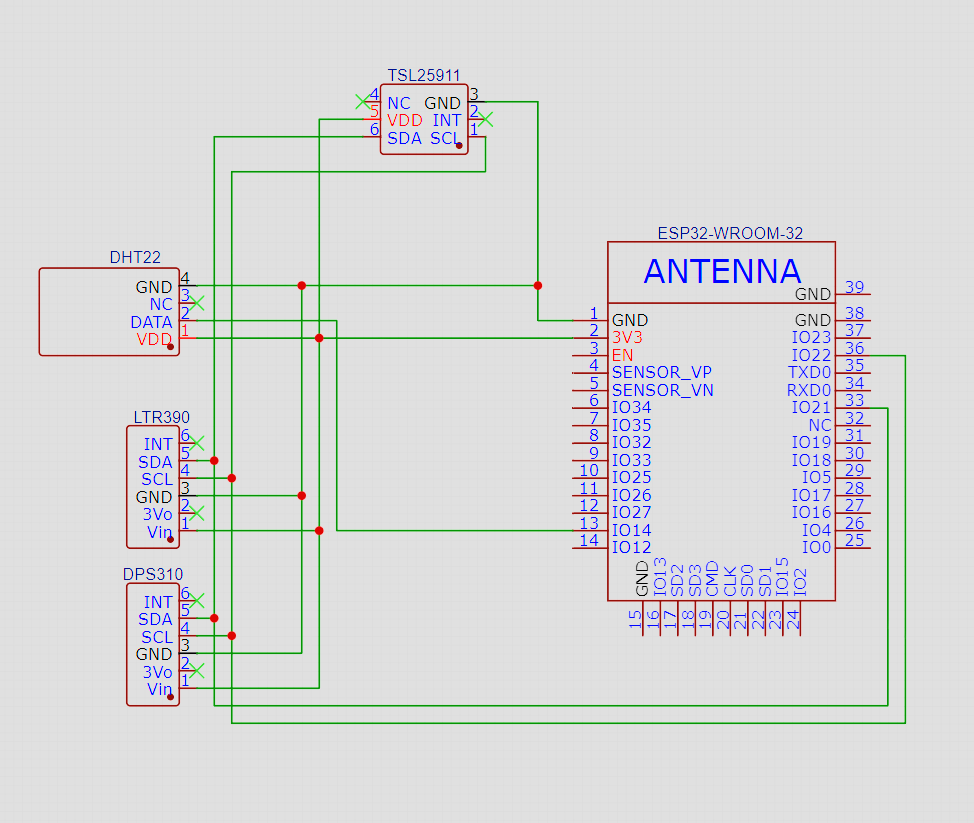
\includegraphics[width=\textwidth]{device-schematic.png}
    \caption{Schemat urządzenia}
    \label{device-schematic}
\end{figure}

\subsection{ESP-WROOM-32}
ESP-WROOM-32 (albo ESP32-WROOM-32) to mikrokontroler ze zintegrowanym WIFI oraz bluetooth. Nadaje się do szerokiej gamy zastosowań:
od kontrolera czujników z niskim poborem energii do zaawansowanych zadań enkodowania sygnałów głosowych czy muzyki. Moduły bazujące na rdzeniach ESP32 zyskały popularność ze wzklędu na zaintegrowaną obsługę WIFI, 
niskim kosztom oraz bogatej dokumentacji oraz wielu możliwych integracji.

Mikrokontroler znajdzie zastosowanie w prostych jak i bardziej skomplikowanych projektach, dzięki dwóm rdzenion, które mogą być kontrolowane osobno,
szerokich możliwościach podłączenia urządzeń perfyferyjnych (wsparcie dla: I2C, UART, SPI oraz inne).

ESP-WROOM-32 składa się z mikrokontrolera ESP32-D0WDQ6 posiadającego dwa rdzenie, które pozwają na prace od 80MHz do 240 MHz. Procesor również
posiada ko-procesor o niskim poborze mocy, który może zostać użyty zamiast głównych rdzeni w przypadku kiedy nie jest potrzebna duża moc obliczeniowa.

Integracja WIFI, Bluetooth i Bluetooth LE do mikrokontrolera pozwala na rozszerzenie możliwych zastosowań, gdzie nie jest możliwe podłączenie do sieci
w konwencjonalny spoób za pomocą kabla. Komunikacja bezprzewodowa również umożliwa całkowicie zdalne zastosowania z wykorzystaniem akumulatorów
oraz paneli słonecznych do zasilania mikrokontrolera.

\subsubsection{Specyfikacja ESP-WROOM-32}

\begin{table}[H]
    \centering
    \begin{tabular}{|l|l|}
        \hline
        Element & Specyfikacja \\
        \hline
        Procesor & 2 rdzenie (80-240MHz) \\
        \hline
        WIFI & 802.11 b/g/n (802.11n: przepustowość 150 Mbps) \\
        \hline
        Bluetooth & Bluetooth v4.2 i Bluetooth LE \\
        \hline
        Pamięć SPI Flash & 4MB \\
        \hline
        Napięcie zasilania & 3.0 V - 3.6 V \\
        \hline
        Zużycie prądu & Średnie: 80 mA \\
        \hline
    \end{tabular}
    \caption{Najważniejsze specyfikacje ESP-WROOM-32}
    \label{esp32-spec}
\end{table}

Do realizacji projektu zostata wybrany mikrokontroler ESP-WROOM-32 ze względu na:
\begin{itemize}
    \item bogate możliwości podłączenia urządzeń perfyferyjnych
    \item wbudowane wspracie połączeń WIFI
    \item dużą ilość pamięci flash
    \item niewielką cenę w porównaniu do oferowanych specyfikacji
    \item łatwą dostępność
\end{itemize}

\noindent Potencjalnymi alternatywami, które nie zostały wybrane do realizacji projektu są:
\begin{itemize}
    \item Arduino Uno R3 (brak wbudowanej obsługi połączeń sieciowych)
    \item ESP8266 (wolniejszy procesor, mniejsza ilość pamięci flash, mniejsza ilość wyprowadzeń do podłączenia urządzeń perfyferyjnych)
    \item Olimex ESP32-POE\cite{olimex-esp32poe} (wbudowana obsługa połączenie przewodowego ethernet, mniejsza ilość wyprowadzeń do podłączenia urządzeń perfyferyjnych)
    \item LILYGO T-SIM7000G\cite{lilygo-esp32lte} (wbudowana obsługa LTE, mniejsza ilość wyprowadzeń do podłączenia urządzeń perfyferyjnych, wysoka cena)
\end{itemize}

\noindent W finalnym produkcie w zależności od przeznaczenia użycie łączności bezprzewodowej może być niewskazane (daleka odległość od punktu dostępowego WIFI, duża ilość przeszkód).
Użycie innych wersji ESP32 z wbudowaną obsługą przewodowego połączenia sieciowego lub możliwościa połączenia do sieci przez LTE, może być wymagane - jednak
w ramach realizacji zakresu projektu wybór padł na łatwiej dostępny moduł z łącznością bezprzewodową WIFI.  

\subsection{Czujnik natężenia światła - TSL25911}

TSL25911 to czujnik światła z odpowiedzią podobną do ludzkiego oka. Posiada czułość 188 uLux oraz zakres dynamiczny 1 do 600,000,000.
W porównaniu do innych tańszych rozwiązań bazujących na fotokomórkach CdS, daje o wiele bardziej precyzujne rezultaty, z możliwością zmiany czułości i
rozdzielczości w locie. 

\subsubsection{Specyfikacja TSL25911}

\begin{table}[H]
    \centering
    \begin{tabular}{|l|l|}
        \hline
        Element & Specyfikacja \\
        \hline
        Rozdzielczość dynamiczna & 1 do 600,000,000 \\
        \hline
        Zakres pomiaru & 188 uLux - 88,000 Lux \\
        \hline
        Zakres temperatury pracy & -30 - 80 °C \\
        \hline
        Interfejs & I2C (adres: 0x29 i 0x28)\\
        \hline
    \end{tabular}
    \caption{Specyfikacja TSL25911}
    \label{tsl25911-spec}
\end{table}

\subsubsection{Przykładowy program testu czujnika TSL25911}

\begin{code}[H]
\inputminted[frame=lines,baselinestretch=1,breaklines,linenos,xleftmargin=1.5em]{c}{../proj/tsl2591-test/tsl2591-test.ino}

\caption{Test czujnika TSL25911}
\end{code}

\subsection{Czujnik temperatury i wilgotności powietrza - DHT22}

Czujnik DHT22 składaja się z dwóch części: pojemnościowego czujnika wilgotności i termistora. 
Wewnątrz znajduje się również bardzo prosty chip, który dokonuje konwersji sygnału analogowego na cyfrowy i wysyła sygnał cyfrowy z temperaturą i wilgotnością. 
Sygnał cyfrowy jest łatwy do odczytania za pomocą dowolnego mikrokontrolera.

Czujnik ten cechuje sie bardzo niską ceną oraz bardzo dużą dokładnością w stosunku do ceny.

Potencjalnymi alternatywami, które mogły być wykorzystane to:
\begin{itemize}
    \item DHT11 (niższa dokładność)
    \item AHT20 (niższa dokładność odczytu temperatury oraz podobna dokładność odczytu wilgotności, dostępny tylko jeden adres I2C)
\end{itemize}

Został wybrany DHT11 ze względu na prostote podłączenia (jedno wyjście cyfrowe) co sprawia, że możliwe jest podłączenie
kilku czujników do jednego mikrokontrolera (co nie możliwe jest w przypadku AHT20, bez wykorzystania na przykład drugigo interfejsu I2C).
Czujnika DHT22 cechuje się również niskim kosztem oraz wysoką dokładność w stosunku do ceny czujnika, co zadecydowało o finalnym wyborze tego produku. 

\subsubsection{Specyfikacja DHT22}

\begin{table}[H]
    \centering
    \begin{tabular}{|l|l|}
        \hline
        Element & Specyfikacja \\
        \hline
        Zakres oraz dokładność odczytu temperatury & -40 to 80 °C (dokładność: 0.5°C) \\
        \hline
        Zakres oraz dokładność odczytu wilgotności & 0 to 100 RH\% (dokładność: 2-5 \%) \\
        \hline
        Maksymalna częstotliwość odczytu danych & 0.5Hz \\
        \hline
    \end{tabular}
    \caption{Specyfikacja DHT22}
    \label{dht22-spec}
\end{table}

\subsubsection{Przykładowy program testu czujnika DHT22}

\begin{code}[H]
\inputminted[frame=lines,baselinestretch=1,breaklines,linenos,xleftmargin=1.5em]{c}{../proj/dht22-test/dht22-test.ino}

\caption{Test czujnika DHT22}
\end{code}

\subsection{Czujnik ciśnienia oraz temperatury - DPS310}

Czujnik DP310 służy do dokładnego pomiaru ciśnienia atmosferycznego oraz posiada dodatkowy czujnik temperatury. Poasiada wysoką dokładność obsolutną +-1 hPa oraz 
pracuje w zakresie od 300 do 1200 hPa. Czujnik cechuje sie niską ceną, wysoką dokładnością w stosunku do ceny, oraz posiada dodatkowy czujnik temperatury, który może 
służyć jako preferowana metoda pomiaru temperatury, albo jako dodatkowy punkt w danych pomiarowych.

Potencjalnymi alternatywami, które mogły być wykorzystane to:
\begin{itemize}
    \item EE895 (niższa dokładność pomiaru ciśnienia (700-1100 hPa, wysoka cena ze względu na obecność czujnika C02))
    \item BMP180 (niższa dokładność pomiaru ciśnienia)
\end{itemize}

Czujnik został wybrany z powodu konkurencyjnej ceny, dużej dostępności oraz wysokiej dokładności pomiaru w stosunku do ceny produktu.

\subsubsection{Specyfikacja DPS310}

\begin{table}[H]
    \centering
    \begin{tabular}{|l|l|}
        \hline
        Element & Specyfikacja \\
        \hline
        Zakres oraz dokładność odczytu temperatury & -40 to 85 °C (dokładność: 1°C) \\
        \hline
        Zakres odczytu ciśnienia atmosferycznego & 300 do 1200 hPa \\
        \hline
        Dokładność absolutna odczytu ciśnienia atmosferycznego & 1 hPa \\
        \hline
        Dokładność dynamiczna odczytu ciśnienia atmosferycznego & 0.002 hPa \\
        \hline
    \end{tabular}
    \caption{Specyfikacja DPS310}
    \label{dps310-spec}
\end{table}

\subsubsection{Przykładowy program testu czujnika DPS310}

\begin{code}[H]
\inputminted[frame=lines,baselinestretch=1,breaklines,linenos,xleftmargin=1.5em]{c}{../proj/dps310-test/dps310-test.ino}

\caption{Test czujnika DPS310}
\end{code}

\subsection{Czujnik światła ultrafioletowego - LTR390}

Czujnik LTR390 jest urządzeniem o bardzo niskim koszcie oraz wysokiej dokładności na światło w zakresie od 300nm do 350 nm. Czujnik posiada dwa sensory - jeden do światła UV, drugi do światła widzialnego 
co pozwala na precyzyjne określenie ilości padającego na czujnik światła UV. W porównaniu do innych czujników oferuje bezpośredni odczyt wartości światła UV z sensora (czujnik SI1145 oblicza ilość światła UV z całkowitego odczytu padającego światłą we wszystkich zakresach) 
oraz pozwala na odczyt dancych za pomocą interfejsu I2C (bez konieczności posiadania interfejsów SPI czy posiadania dodatkowych konwerterów analogowo-cyfrowcych) 

Potencjalnymi alternatywami, które mogły być wykorzystane to:
\begin{itemize}
    \item SI1145 (niższa dokładność pomiaru światła UV - brak bezpośreniego odczytu - wartość oblicznana)
    \item GUVA-S12SD (wymagany konwerter analogow-cyfrowy do odczytu danych)
\end{itemize}

Czujnik został wybranu z powodu wysokiej dokładności (bezpośredni odczyt wartości padającego światła UV) oraz prostoty podłączenia czujnika do mikrokontrolera (interfejs I2C). 
Bardzo niska cena oraz możliwość odczytu natężenia światła (w lux) jest dodatkowym plusem.

\subsubsection{Specyfikacja LTR390}

\begin{table}[H]
    \centering
    \begin{tabular}{|l|l|}
        \hline
        Element & Specyfikacja \\
        \hline
        Zakres odczytu światła UV & od 300nm do 350nm \\
        \hline
        Zakres odczytu światła widzialnego & od 0 do 524287 (20 bitowy zakres) \\
        \hline
        Interfejs & I2C (adres: 0x53) \\
        \hline
    \end{tabular}
    \caption{Specyfikacja LTR390}
    \label{ltr390-spec}
\end{table}

\subsubsection{Przykładowy program testu czujnika LTR390}
\begin{code}[H]
\inputminted[frame=lines,baselinestretch=1,breaklines,linenos,xleftmargin=1.5em]{c}{../proj/ltr390-test/ltr390-test.ino}

\caption{Test czujnika LTR390}
\end{code}

\section{Środowisko programowe}
Do implementacji systemu wbudowanego wykorzystane zostaną:
\begin{itemize}
    \item Język C do utworzenia oprogramowania mikrokontrolera
    \item Język HTML oraz CSS do utworzenia interfejsu www
    \item Środowisko programistyczne Arduino Studio w wersji 2.2.1
\end{itemize}

\section{Oprogramowanie}

\subsection{Protokół mDNS}

Protokół mDNS służy do rozwiązywania nazw urządzeń sieciowych do adresów IP - dzięki temu użytkownik ma możliwość połączenia z urządzeniem nie znając
jego adresu - wystarczy nazwa urządzenia sieciowego. mDNS należy do rodziny protkołów Zeroconf (lub zero-config)\cite{zeroconf-explanation} - nie wymaga konfiguracja do pracy 
i jest protkół ten wspierany przez Windowsa (10+) oraz Linuxa (po instalacji programu Avahi).

W projekcie zostanie protokół ten użyty, aby użytkownik nie musiał znać adresu IP urządzenia, aby sie z nim połączyć. 
Protokół jest konfigurowany za pomocą pliku nagłówkowego \texttt{ESPmDNS.h}. Aby skonfigurować usługę, aby mikrokontroler był możliwy do odnalezienia
w sieci poprzez mDNS nalezy wystartować serwer mDNS oraz dodać nową usługę usługę z typem (w przykładzie \texttt{http}), protkołem (w przykładzie \texttt{tcp}) 
oraz portem pod którym usługa jest dostępna (w przykładzie: \texttt{80} - port serwera www z danymi, które udostępnia urządzenie).

Po prawidłwej konfiguracji oraz wpisaniu adresu \\\texttt{http://esp32-weather-station.local/} w przeglądarce powinniśmy zobaczyć stronę www udostępnianią przez
mikrokontroler.

\begin{code}[H]
\begin{minted}[frame=lines,baselinestretch=1,breaklines,linenos,xleftmargin=1.5em]{c}
void setup()
{
    // esp32-weather-station.local
    if (!MDNS.begin("esp32-weather-station")) {
        Serial.println("Error setting up MDNS responder!");
        while (1) {
        delay(1000);
        }
    }

    MDNS.addService("http", "tcp", 80);
}
\end{minted}
\caption{Przykład konfiguracji usługi mDNS}
\end{code}

Do implementacji serwera http została użyta biblioteka ESP32 HTTPS Server \cite{esp32-https-server-library}. 

\begin{code}[H]
\begin{minted}[frame=lines,baselinestretch=1,breaklines,linenos,xleftmargin=1.5em]{c}
#include <HTTPServer.hpp>
#include <HTTPRequest.hpp>
#include <HTTPResponse.hpp>

httpsserver::HTTPServer http_server = httpsserver::HTTPServer();

void handle_api_request(
    httpsserver::HTTPRequest *req, 
    httpsserver::HTTPResponse *res
);
void handle_root_request(
    httpsserver::HTTPRequest *req, 
    httpsserver::HTTPResponse *res
);

void setup(void)
{
    httpsserver::ResourceNode *nodeRoot = new httpsserver::ResourceNode(
        "/", 
        "GET", 
        &handle_root_request
    );
    httpsserver::ResourceNode *nodeApi = new httpsserver::ResourceNode(
        "/api", 
        "GET", 
        &handle_api_request
    );
    http_server.registerNode(nodeRoot);
    http_server.registerNode(nodeApi);
    http_server.start();
    if (http_server.isRunning()) {
        Serial.println("Server ready.");
    }
}

void loop(void)
{
    http_server.loop();
}
\end{minted}
\caption{Wycinek kodu konfigurującego serwer http}
\label{http-server-code-parts}
\end{code}

Biblioteka pozwala na proste definiowanie adresów podstron, wraz z przyjmowanym typem zapytania http. Gdy serwer http odbierze zapytanie o
podstrone z prawidłowym adresem, wykonuje metode zarejestrowaną w obiekcie serwera.

\subsection{Dostęp do danych przez przeglądarkę}

Urządzenie udostępnia stronę www z odczytami czujników w prostym formacie dla odczytu przez człowieka. 
Przy pomocy HTML oraz CSS prezentowana jest tabela ze wszystkimi danymi, które udostępnia urządzenie, informacja jaki czas temu
dane były aktulizowane oraz jak długo urządzenie pracuje.

Aktualne dane zebrane przez urządzenie są wstrzykiwane do szablonu http za pomocą funkcji \texttt{sprintf}. W pierwszym parametrze podana jest
zmienna do bufora na przetwarzane, w drugim zmienna z szablonem html a reszta parametrów to poszczególne dane, które mają być wstrzyknięte.
Następnie gotowy plik html jest wysyłany do użytkownika.

\begin{code}[H]
\begin{minted}[frame=lines,baselinestretch=1,breaklines,linenos,xleftmargin=1.5em,samepage]{c}
void handle_root_request(
    httpsserver::HTTPRequest *req, 
    httpsserver::HTTPResponse *res
) {
    res->setHeader("Content-Type", "text/html");

    char buffer[2000];
    sprintf(
        buffer, 
        html_template,
        mdns_hostname,
        mdns_hostname,
        current_reading_data.temperature,
        current_reading_data.humidity,
        current_reading_data.heat_index,
        current_reading_data.visible_light,
        current_reading_data.full_spectrum_light,
        current_reading_data.infrared_light,
        current_reading_data.calculated_lux,
        current_reading_data.pressure,
        current_reading_data.uvs,
        sensor_read_delay,
        calculate_uptime()
    );

    res->print(buffer);
}
\end{minted}
\caption{Kod obsługujący interfejs użytkownika}
\label{user-interface-code}
\end{code}

Szablon pliku html jest przechowywany w pamięci programowej programu w stałej \texttt{html\_template}. Zaletą takiego rozwiązania jest prostota implementacji
oraz szybkość działania - dane są zawsze gotowe do wykrzystania. Alternatwywnie można byłoby wykorzystać pamięć SPIFFS urządzenia do przechowywania szablonu
html - byłoby to bardziej elastyczne rozwiązanie, które nie wymagało by ponownej kompilacji programu, aby zmienić szablon html. Z drugiej strony rozwiązanie to
mogłoby powodować zwiększony narzut przy generowaniu odpowiedzi przy każdym zapytaniu. Ze wzlędu na prostotę pierwszego rozwiązania oraz potencjalne
problemy z wydajnością drugiego rozwiązania zdecydowałem sie załadować szablon do kodu programu w tej wersji oprogramowania.
Do deklaracji zawartości zmiennej jest użyta deklaracja literał ciągu znaków (string literal), aby w prosty sposób było możliwe zawarcie w środku 
zmiennej znaków spcjalnych, znaków niedozwolonych oraz w celu Udostępnienia możliwości deklaracji wieloniowego ciągu znaków.

\begin{code}[H]
\begin{minted}[frame=lines,baselinestretch=1,breaklines,linenos,xleftmargin=1.5em]{c}
const char html_template[] = R"###(
    <html lang="en">
    <head>
    ...
)###";
\end{minted}
\caption{Kod deklaracji szablonu html}
\label{html-template-code}
\end{code}

Przyszłym usprawnieniem urządzenia mogłoby być sprawdznie wydajności pamięci SPIFFS do przechowywania szablonów html, aby oszczedzić na pamięci programowej. 

\subsection{Dostęp do danych przez REST API}

Urządzenie udostępnia dane również poprzez REST API w postaci JSON - umożliwia to łatwą integrację urządzenia z innymi narzędziami, 
albo umożliwia stworzenie własnych integracji. 

\subsection{Dostęp do danych diagnostycznych}

Urządzenie udostępnia dane, które mogą słuzyć do debugowania urządzenia za pomocą interfejsu szeregowego. W przypadku wykorzystanego w projekcie
mikrokontrolera po uruchomieniu urządzenia dane zostaną wysyłane również na port szeregowy oprócz reszty procesów do przetwarzania danych.

Funkcja \texttt{send\_debug\_info\_to\_serial} wysyła dane na interfejs szeregowy w postaci łatwej do przeczytania dla człowieka:

\begin{code}[H]
\begin{minted}[frame=lines,baselinestretch=1,breaklines,linenos,xleftmargin=1.5em]{c}
void send_debug_info_to_serial()
{
    Serial.print(F("DHT22 sensor data - Temp: '"));
    Serial.print(current_reading_data.temperature);
    Serial.print(F("' Humidity: '"));
    Serial.print(current_reading_data.humidity);
    Serial.print(F("' Heat index: '"));
    Serial.print(current_reading_data.heat_index);
    Serial.println(F("'"));

    Serial.print(F("TSL2591 sensor data - Calculated Lux: '"));
    Serial.print(current_reading_data.calculated_lux);
    Serial.print(F("' Full spectrum light: '"));
    Serial.print(current_reading_data.full_spectrum_light);
    Serial.print(F("' Infrared light: '"));
    Serial.print(current_reading_data.infrared_light);
    Serial.print(F("' Visible light: '"));
    Serial.print(current_reading_data.visible_light);
    Serial.println(F("'"));

    Serial.print(F("DPS310 sensor data - Pressure: '"));
    Serial.print(current_reading_data.pressure);
    Serial.println(F("hPa'"));

    Serial.print(F("LTR390 sensor data - UVS: '"));
    Serial.print(current_reading_data.uvs);
    Serial.println(F("'"));

    Serial.println(F(""));
}
\end{minted}
\caption{Kod dostępu do danych diagnostycznych}
\label{diagnostic-data-code}
\end{code}

Jako, że powyższa funkcja operuje na dużej ilość tekstu w sposób cały, zostało zastosowana optymalizacja w postaci użycia funkcji 
\texttt{F} - funkcja ta sprawia, że dany łańcuch znaków nie jest kopiowany do pamięci PSRAM mikrokontrolera przed wysłaniem na interfejs szeregowy, 
a dane są beźpośrednio kopiowane z programu do strumienia, który wysyłane dane na interfejs. 

\subsection{Integracja z MQTT}

Urządzenie dodatkowo udostępnia możliwość połączenia do serwera MQTT - co umożliwia bezpieczne udostępniane danych do serwera zewnętrzengo.
Do implementacji połączenia do serwera MQTT użyta została biblioteka \texttt{EspMQTTClient}\cite{esp32-mqtt-server-library} - 
zarządza połączeniem do serwera oraz wymianą danych między klientem oraz serwerem.

Poniższy kod umożliwia podłączenie urządzenia do lokalnego albo zewnętrzego serwera MQTT: 
\begin{code}[H]
\begin{minted}[frame=lines,]{c}
void send_debug_info_to_serial()
EspMQTTClient mqtt_client(
    "192.168.0.15", // host
    1883, // port
    "username", // username
    "password", // password
    mdns_hostname // device name
);
\end{minted}
\caption{Kod dostępu do danych diagnostycznych}
\label{diagnostic-data-code}
\end{code}

\section{Testy}

\subsection{Interfejs WWW}
Interfejs WWW użytkownika zawiera komplet danych zbieranych przez urządzenie oraz kiedy ostatni raz dane były aktualizowane. 
Odświeżenie przeglądarki spodowuje pobranie nowych danych z urządzenia.
\begin{figure}[H]
    \centering
    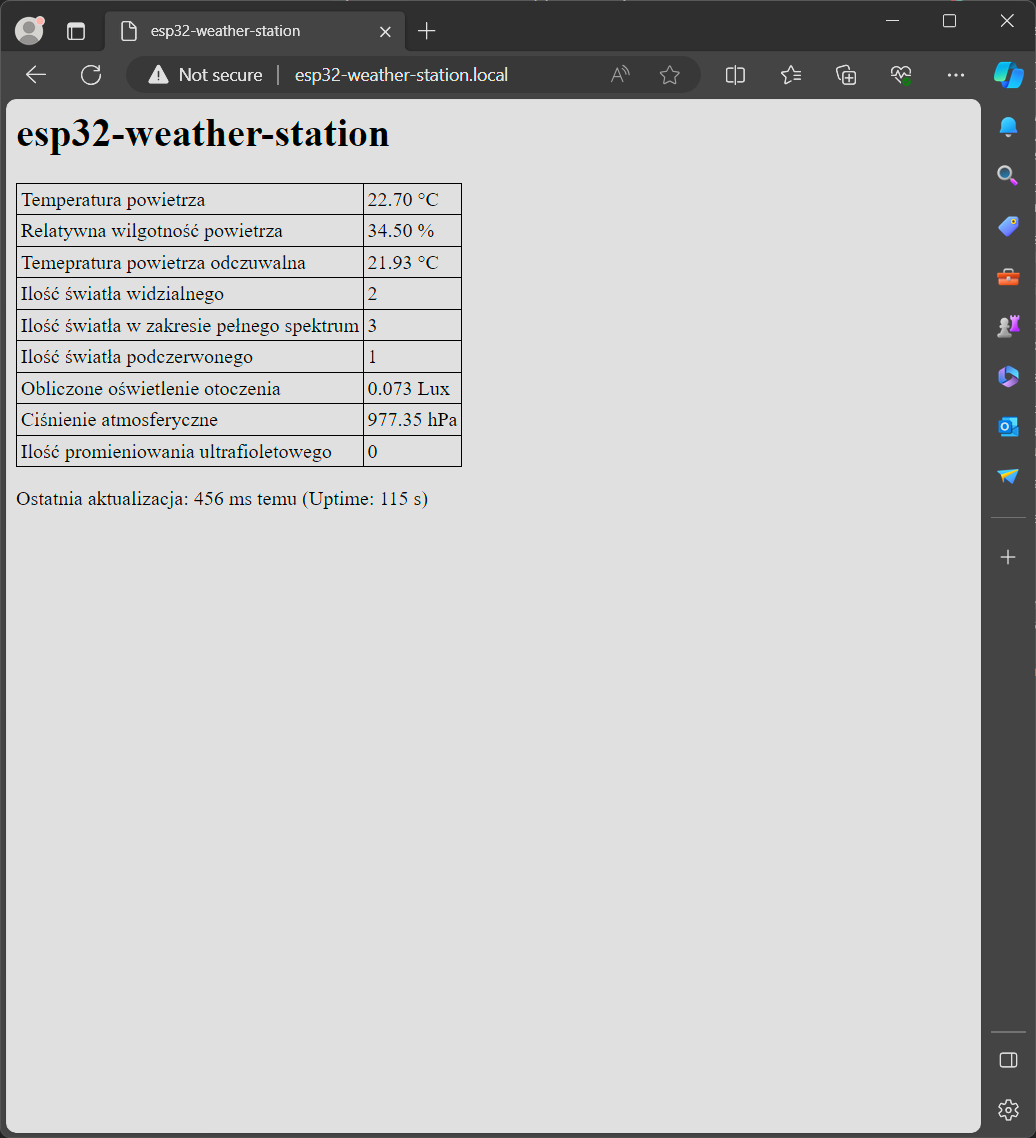
\includegraphics[width=\textwidth]{web-interface.png}
    \caption{Test interfejsu WWW}
\end{figure}

\subsection{Interfejs REST API}
Interfejs REST dla programisty zwraca dane w formacie JSON.
\begin{figure}[H]
    \centering
    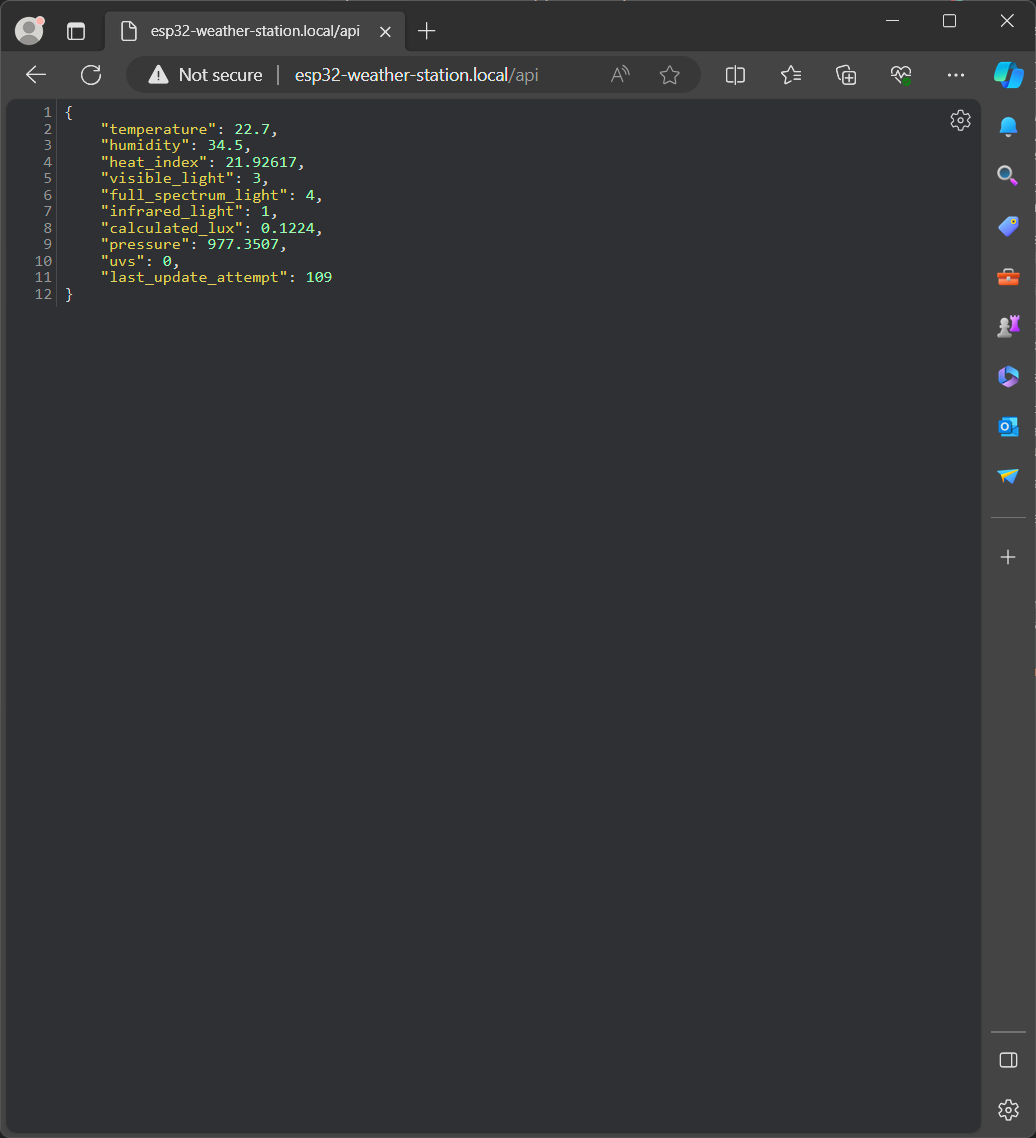
\includegraphics[width=\textwidth]{rest-api.png}
    \caption{Test interfejsu REST API}
\end{figure}

\subsection{MQTT}
Urządzenie dodatkowo wysyła dane z czujników do skonfigurowane serwera MQTT. Dane są wysyłane od razu po ich aktualizacji.
\begin{figure}[H]
    \centering
    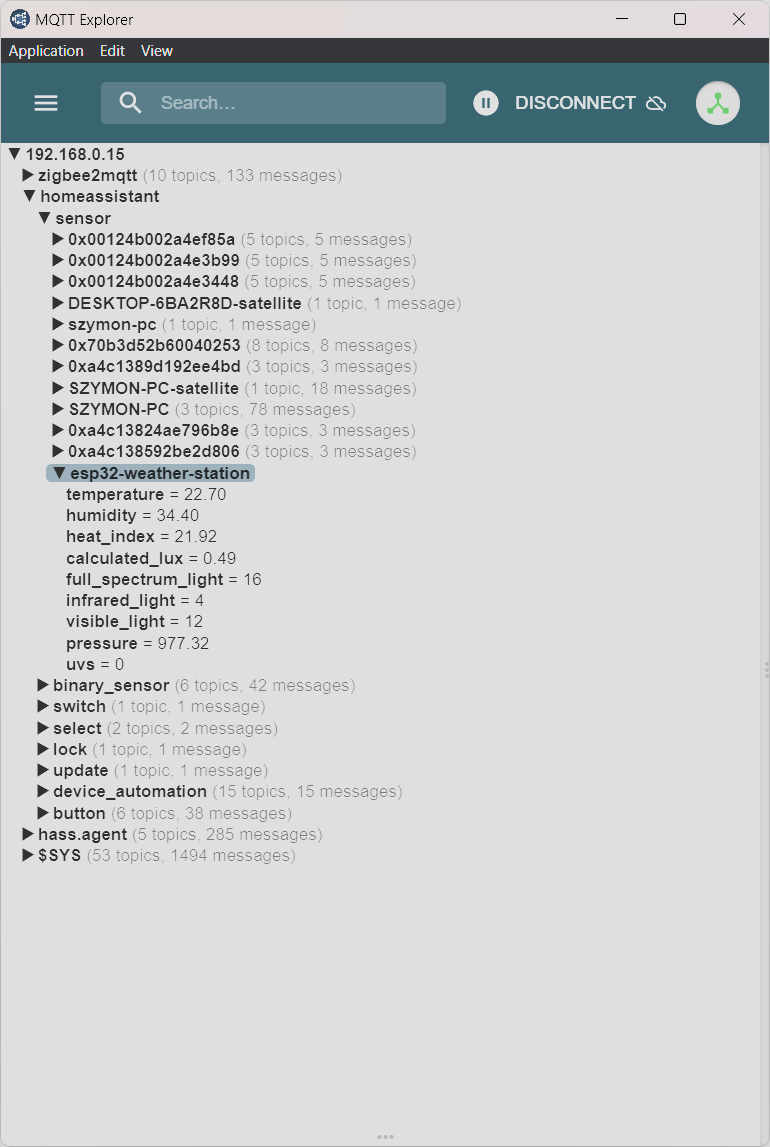
\includegraphics[width=\textwidth]{mqtt1.png}
    \caption{Test integracji z MQTT}
\end{figure}

\subsection{Porównanie z komercyjnymi danymi pogodowymi}

Dane pogodowe dostarczane przez urządzenie będą bardziej dokładne lokalnie niż prognoza pogody dostępna 
w komercyjnych serwisach. Obrazek \ref{test-outside-site} wykazuje, że aktualna temperatura wynosi 
\texttt{-3.6°C} a względna wilgotność powietrza wynosi \texttt{73.7\%}. 
Dane udostępniane przez serwis meteo.pl \cite{meteopl-nysa} dla tej samej co lokalizacja urządzenia
wskazuje, że temperatura wynosi 
\texttt{-5°C} a względna wilgotność powietrza wynosi \texttt{85\%}.

\begin{figure}[H]
    \centering
    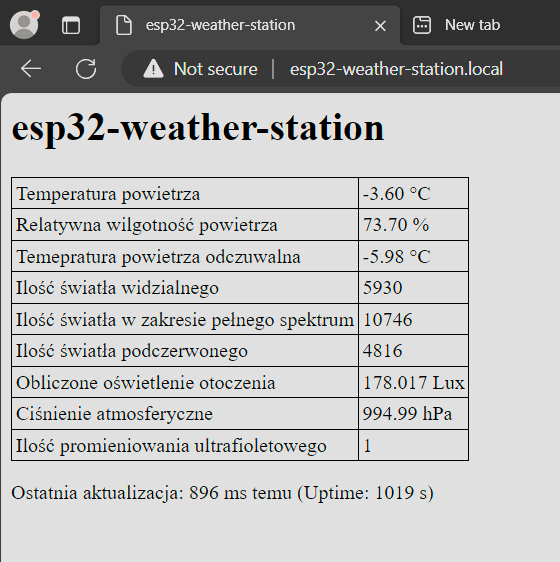
\includegraphics[width=\textwidth]{test-outside-site.png}
    \caption{Porównanie danych pogodowych - urządzenie}
    \label{test-outside-site}
\end{figure}

\begin{figure}[H]
    \centering
    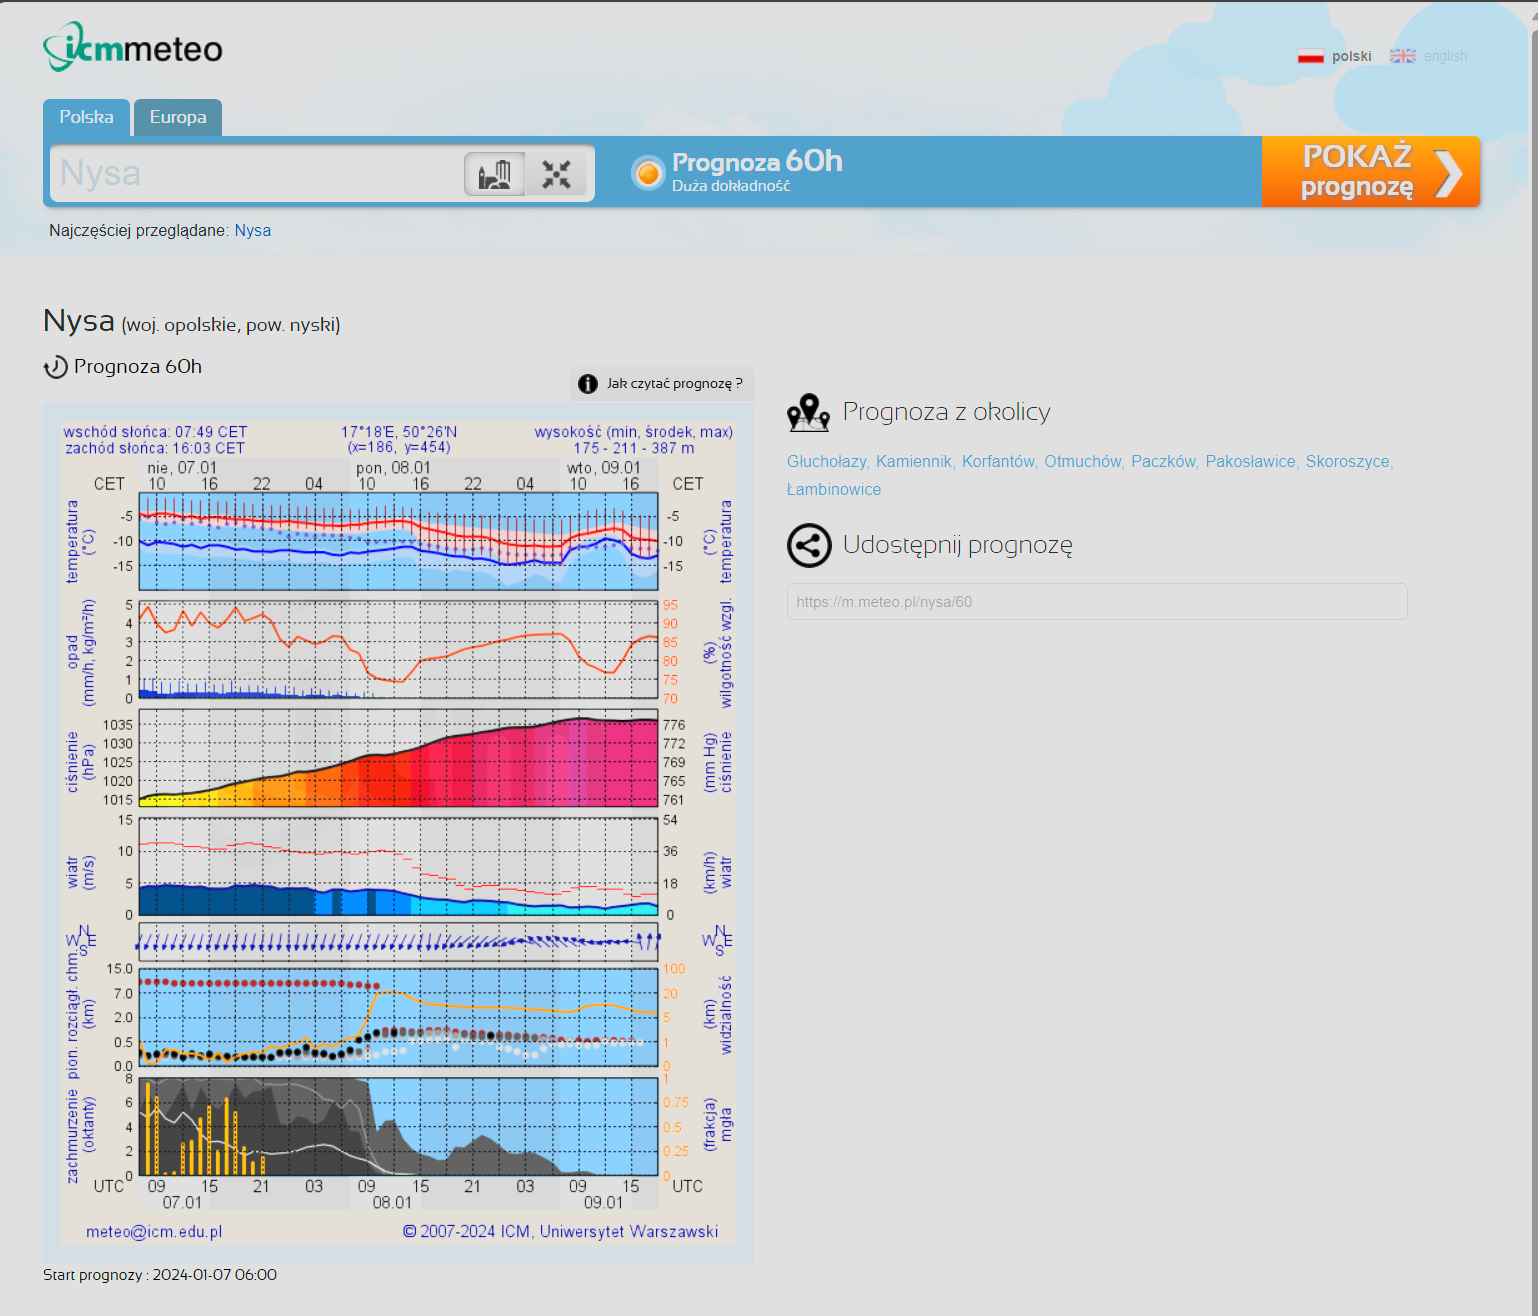
\includegraphics[width=\textwidth]{test-outside-meteo.pl.png}
    \caption{Porównanie danych pogodowych - meteo.pl}
    \label{test-outside-meteo}
\end{figure}

\subsection{Dostęp do danych za pomocą MQTT i Home Assistant}

Dane przesyłane do MQTT mogą być odczytane przez zewnętrzny serwis w ceu wyświetlenia danych - w tym przypadku jest to aplikacja Home Assistant\cite{homeassistant}. Za pomocą wpisu w konfiguracji w języku
YAML możliwe jest odczytanie danych z serwera MQTT i wyświetlenie danych tych na panelu. 

\begin{figure}[H]
    \centering
    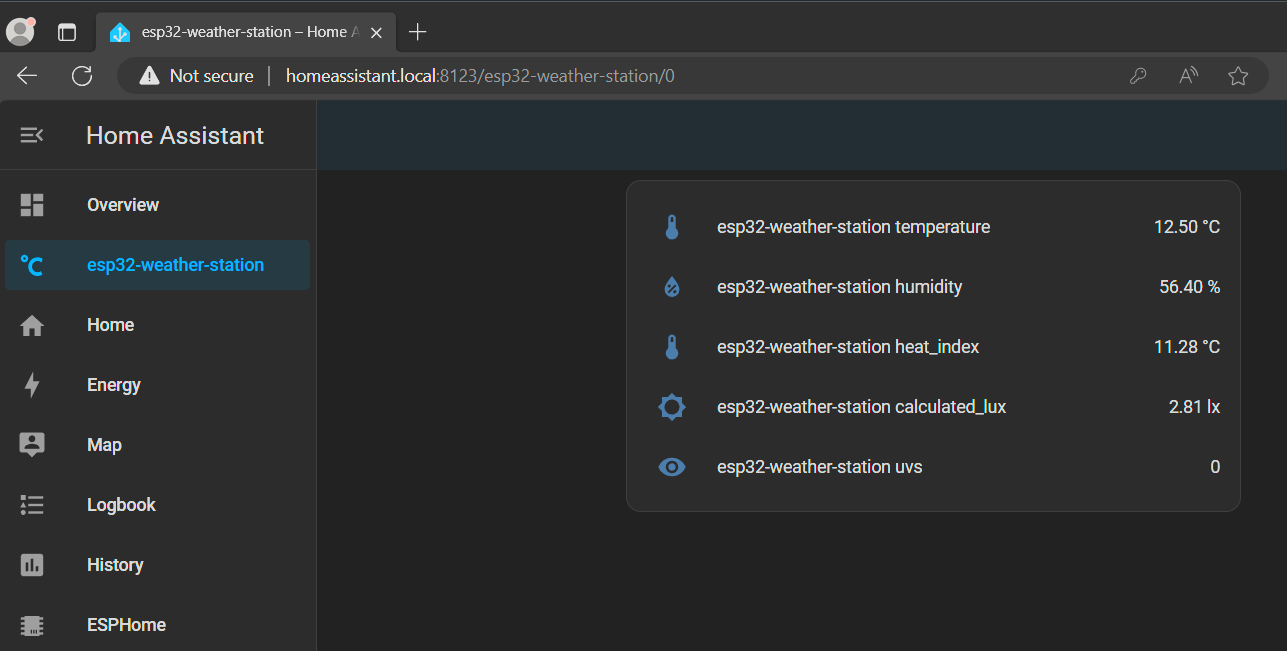
\includegraphics[width=\textwidth]{home-assistant-weathe-station.png}
    \caption{Dostęp do danych pogodowych przez Home Assistant}
    \label{homeassistant-weather-station}
\end{figure}

\section{Wnioski}
Moduły bazujące na mikrokontrolerze ESP32 pozwalają na łatwą realizację projektów, a przez dużą różnorodność
dostępnych na rynku modułów bazująych na tym mikrokontrolerze daje to ogromną wszechstronność w realizacji oraz dostępności, jednocześnie zachowując kompatybilność między modułami.

W tej pracy zrealizowana lokalna stacja pogodowa umożliwia odczyt danych pogodowych w sieci lokalnej a także umożliwia łatwą integrację z zewnętrzymi systemami (interfejs REST API oraz integracja z MQTT).

Dostęp do danych spoza sieci lokalnej możliwy jest po podłączeniu do dostępnego publicznie serwera MQTT - urządzenie zostaje dostępne tylko w sieci lokalnej i nie jest narażone na potencjalne ataki w przypadku jeżeli urządzenie te byłoby dostępne publicznie. Lokalny dostęp do urządzenia jest jest bardzo prosty dzięki protokołowi mDNS - aby połączyć się z urządzeniem nie jest potrzebny adres IP, a wystarczy nazwa urządzenia w sieci, która jest statyczna.

Kolejnym etapem rozwoju projektu mogłabybyć kolejna wersja interfejsu użytkownika, dodatkowe integracje z innymi systemami zewnętrzynymi lub integracja czujników oraz mikrokontrolera na jednej płytce PCB.

Podłączenie kolejnych czyjników do urządzenia również nie powinno sprawiać problemu ze względu na dużą dostępność dodatkowyć pinów WE/WYJ oraz
otwartej nartury całego ekosystemu Arduino. 

\section{Literatura}

\printbibliography[heading=none]

\section{Spisy programów, tabel, fotografii}
\listoftables
\listof{code}{Spis programów}
\listoffigures

\section{Streszczenie}
Praca inżynierska podejmuje temat "Konstrukcja stacji pogodowej opartej na mikrokontrolerze ESP32 z interfejsem użytkownika oraz API REST". Głównym celem pracy było przygotowanie prototypu urządzenia stacji pogodowej wraz z oprogramowaniem oraz test przydatności takiego urządzenia do celów domowych. W ramach pracy został wybrany mikrokontroler oraz czujniki wykorzystane w urządzeniu. 
Zostało przygotowane również oprogramowanie, które steruje pracą mikrokontrolera - urządzenia udostępnia interfejs www dla użytkownika, interfejs programowy REST API oraz integracje z MQTT. Duża różnorodność czujników, wysoka dostępność mikrokontrolerów oraz bogaty ekosystem programowy umożliwia szybką, tanią i prostą konstrukcje urządzeń bazujących na ESP32. Zaletami lokalnej stacji pogodowej jest wysoka dokładność oraz wysoka przewidywalność odczytów w porównaniu do danych zbieranych przez inne komercyjne serwisy.

\end{document}
